\documentclass[10pt]{llncs}

\usepackage{doc}
\usepackage{makeidx}
\usepackage{fancyvrb}
\usepackage{listings}
\usepackage{longtable}
\usepackage{paralist}
\usepackage{color}
\usepackage{algpseudocode}
\usepackage{hyperref}
\usepackage{graphicx}
\usepackage{mathtools}
\usepackage{amsfonts}
\usepackage{stmaryrd}
\usepackage{amsmath}
\usepackage{verbatim}
\usepackage{txfonts}
\hypersetup{
    colorlinks,
    citecolor=black,
    filecolor=blue,
    linkcolor=black,
    urlcolor=blue
}
% for overriding caption view
\usepackage{caption}
\captionsetup[lstlisting]{ singlelinecheck=false, margin=0pt, font={it,footnotesize} }

% Let's style the code!
% Set-up code visualisation
\lstset{fancyvrb=true}
\lstset{
language=java,                  % the language of the code
basicstyle=\footnotesize,       % the size of the fonts that are used for the code
numbers=left,                   % where to put the line-numbers
numberstyle=\footnotesize,      % the size of the fonts that are used for the line-numbers
stepnumber=1,                   % the step between two line-numbers. If it's 1, each line 
                                % will be numbered
numbersep=5pt,                  % how far the line-numbers are from the code
keywordstyle=\color{blue},
commentstyle=\color{green},
stringstyle=\color{red},
backgroundcolor=\color{white},  % choose the background color. You must add \usepackage{color}
showspaces=false,               % show spaces adding particular underscores
showstringspaces=false,         % underline spaces within strings
showtabs=false,                 % show tabs within strings adding particular underscores
frame=single,                   % adds a frame around the code
tabsize=2,                      % sets default tabsize to 2 spaces
captionpos=t,                   % sets the caption-position to bottom
breaklines=true,                % sets automatic line breaking
breakatwhitespace=false,        % sets if automatic breaks should only happen at whitespace
%title=\lstname,                 % show the filename of files included with \lstinputlisting;
                                % also try caption instead of title
escapeinside={\%*}{*)},         % if you want to add a comment within your code
morekeywords={*,...}            % if you want to add more keywords to the set
}
\lstset {
    keywordstyle=\color[rgb]{0,0,1},          % keywords in blue
    commentstyle=\mcommentfont,               % comments
    stringstyle=\color[rgb]{.627,.126,.941},  % strings in purple
    commentstyle=\color[rgb]{.133,.545,.133}
}

% In order to save space or manage large tables or figures in a
% landcape-like text, you can use the rotating and pdflscape
% packages. Uncomment the desired from the below.
%
% \usepackage{rotating}
% \usepackage{pdflscape}

% If you plan on including some algorithm specification, we recommend
% the below package. Read more details on the custom options of the
% package documentation.
%
% \usepackage{algorithm2e}

%\makeindex

%% Document
%%


% Regular title as in the article class.
\title{Ensuring Faultless Communication Behaviour\\
       in an E-Commerce Cloud Application}

% \titlerunning{} has to be set to either the main title or its shorter
% version for the running heads.
\titlerunning{Faultless Communication in a Cloud}

% Authors are joined by \and. Their affiliations are given by \inst, which indexes
% into the list defined using \institute
\author{
	Rustem A. Kamun \and Ross Horne
}

% Institutes for affiliations are also joined by \and,
\institute{
  Kazakh-British Technical University, 
  Faculty of Information Technology,\\
  Almaty, Kazakhstan\\
  \email{r.kamun@gmail.com}
}

%  \authorrunning{} has to be set for the shorter version of the authors' names.
\authorrunning{R. Kamun \& R. Horne}

\begin{document}

%%%%%%%%%%%%%%%%%%%%%%%%%%%%%%%%%%%%%%%%%%%%%%%%%%%
\maketitle
%%%%%%%%%%%%%%%%%%%%%%%%%%%%%%%%%%%%%%%%%%%%%%%%%%%

\begin{abstract}
The scale and complexity of Web Services raises the challenge of controlling their interaction. The goal of this work is to ensure that processes in a Cloud are correctly interacting according to a specification of their communication behaviour. To accomplish this goal, we employ session types to analyse the global and local communication patterns. Session types represents ``formal blueprints" of how communicating participants should behave and offers a concise view of the message flows.
  
This work confirms the feasibility of application of session types on business protocols used by an e-commerce Cloud provider and developed in Session-Java, an extension of Java implementing Session-Based programming. Furthermore, we highlight the importance of this approach for services replicated across multiple Cloud providers each of which must correctly cooperate.
\end{abstract}

\setcounter{tocdepth}{2}
%\small\tableofcontents}

\pagestyle{empty}


%------------------------------------------------------------------------------
\section{Introduction}
\label{sect:introduction}

%The growing needs for information availability and accessibility present new challenges for application development.
The need for distributed highly available services presents challenges for application development.
%Two forces working in parallel with regards to the need for integration.
It is necessary for applications to be integrated both within an enterprise, and between businesses.
Service-Oriented Architectures (SOA) are widely accepted as a paradigm for integrating software applications within and across organizational boundaries.
In this paradigm, independently deployed applications are exposed as Web Services which are then 
interconnected using a stack of standards. %(depicted in Figure~\ref{fig:soa-stack}). 
		
It is challenging to managing service interactions that go beyond simple sequences of requests and responses or involve large numbers of participants (multi-party communication).
%A need arises for new transaction implementations, more suitable for the Web.
One technique for describing collaboration between a collection of services is a choreography.
Choreographies capture a global view of the interactions between participating services. % engage and interconnections between these interactions, including control-/data-flow dependencies.
However, a choreography does not specify how a global description can be executed.
%However, a choreography does not describe internal effects within a participating service.

%, and, therefore, its functionality is not clear.
\begin{comment}
		\begin{figure}[ht]
		\begin{centering}
		\scalebox{0.7}{
		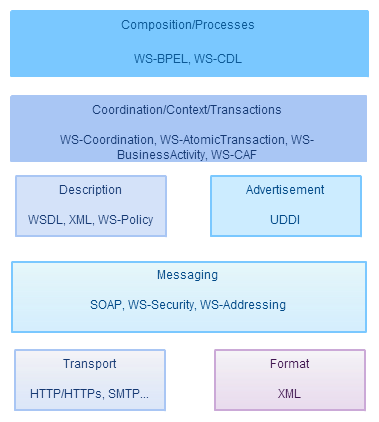
\includegraphics[width=0.5\textwidth]{resources/WS_stack.png}
                }
		\caption{Stack of WS Standards}
		\label{fig:soa-stack}
		\end{centering}
		\end{figure}
\end{comment}

%Applications include business transactions operating in closely coupled context (e.g.\ the online stock exchange (ForEX), and e-commerce services based on Buyer-Seller-Shipper (BSH) protocols).
%Highly available services are likely to have a long life span that may result in deadlock.
%Although,in closely coupled settings, the SOA standards may incur a significant performance overhead.

%In addition there is no special concept of the participants of communication. 

\begin{comment}
	\begin{compactenum}
	   \item business transactions with short life span, operating in closely coupled context, where SOA standards may become a trap (online stock exchange(ForEX), services based on BSH protocol\footnote{Buyer-Seller-Shipper protocol} such as e-commerce services);
	   \item applications with a long life span that may result in deadlock.
	\end{compactenum}
\end{comment}

%The concept of a participant in a communication is essential in complex interactions.
%Much literature exist on the specification of systems that describe services from the local perspective of a participant~\cite{cs-processes,alg-seq-processes,Milner1992}.
The challenge of controlling interactions of participants motivated the design of Web Services Choreography Description Language (WS-CDL)~\cite{session-types-sessions}.
The WS-CDL working group identified critical issues~\cite{ws-critical-overview} including:
\begin{compactenum}
	\item the need for tools to validate conformance to choreography specifications to ensure correct cooperation between Web Services;
	\item design time validation and verification of choreographies to guarantee correctness of such properties like deadlock, livelock e.g.\ behaviour of participants conforms to the choreography interface.
\end{compactenum}

The aforementioned challenges can be tackled by adopting a solid foundational model. Successful approaches based on session types~\cite{session-types-sessions,carbone2007structured} include: the Chor and Jolie programming languages of Carbone and Montesi~\cite{chor-lang,carbone2013deadlock} based on sessions and trace sets~\cite{chor-essence}; Session-Java~\cite{sj-lang}, Scribble~\cite{honda2011scribbling} and Session C~\cite{ng2012multiparty} due to Honda and Yoshida; Sing\#~\cite{basu2012deciding} that extends Spec\# with choreogrphies; and UBF(B)~\cite{armstrong2002getting} for Erlang.

In this paper, we demonstrate a method of controlling process interactions represented by sessions. The formal theory based on session types ensures communication safety by verifying that session implementations of each engaged participant conform to the defined protocol specification. In order to evaluate the feasibility of this theory we use Session-Java, an extension to Java language. Session Java works by specifying the intended process transaction protocol using session types and implementing the interaction using session operations.

%Through these we are aiming to confirm the suitability of Session-Java as an implementation of business to business transactions. We want to explore the agility and robustness of the language and the scalability as scenarios vary in size but also complexity. In addition we will be looking for things such as ease of programming in SJ, any limitations, bugs or non-implementable scenarios.


In Section~\ref{sect:basics} we provide an overview of SJ.
In Section~\ref{sect:impl}, we explain several refinements of protocols used by a Cloud provider, using SJ. %and how they can be implemented correctly using session programming.
Finally, in Section~\ref{sect:highlights}, we highlight how session types can improve the design of InterCloud~\cite{intercloud} communication protocols.


%------------------------------------------------------------------------------
\section{Basics of Session-Java}
\label{sect:basics}

We briefly outline how Session-Java is employed to correctly implement protocols.
%Session programming can be applied when participants cooperate according to specified protocols.
%Session types are formal specifications of protocols, that describe structured sequences of interaction including basic message passing, branching and recursion.
Firstly, the global protocol is specified using sequence diagrams. The global specification is projected to sessions types, which specify the protocol for each participant.
The session is then implemented using operations on session sockets. The correctness of the protocol can be verified using session types.

%according to the protocol using Session programming begins from the protocols specification for interaction (using session types), which can then be concretely implemented using structured communication operations available on session sockets.


\begin{comment}
A session is an instance of a session type, i.e.\ the unit of interaction encapsulating one run of a protocol. From the perspective of abstraction, each session, is conducted on a separate channel. 

Session programming in SJ consists of the following ordered actions:

\begin{compactenum}
  \item design specification (protocol) of target communication;
  \item mapping protocols into the programs for each participant. For instance, in BSH protocols, we can distinguish three main participants whose actions (processes) are mapped to corresponding programs (software component);
  \item By utilizing session programming constructs, implementing the protocol, where each operation is performed as method call;
  \item verification of sessions fulfilment by  compiler;
  \item execution and system testing.
\end{compactenum}
\end{comment}


\begin{figure}
\begin{gather*}
\begin{array}{c}
L_1, L_2\quad\mbox{tag}
\\[10pt]
p\quad\mbox{protocol name}
\\[10pt]
M \Coloneqq \textit{Datatype} \mid T \quad\mbox{message}
\\[10pt]
S \Coloneqq  p\left\{ T \right\} \quad \mbox{session}
\end{array}
\qquad
\begin{array}{rlr}
T \Coloneqq & T\mathbin{.}T & \mbox{Sequencing} \\ 
       \mid & \texttt{begin} & \mbox{Session initiation} \\
       \mid & \mathopen{!}\left<M\right> & \mbox{Message send} \\ 
       \mid & \mathopen{?}\left(M\right) & \mbox{Message receive} \\
       \mid & \left\{L_1 \colon T_1,\dots, L_n \colon T_n \right\} & \mbox{Session branching} \\ %??Why not use the ASCII syntax, since you use it in examples. was \oplus \left\{L_1 \colon T_1,\dots, L_n \colon T_n \right\}
       \mid & \left[T\right]* & \mbox{Session iteration} \\ 
       \mid & \texttt{rec}\,L\left[T\right] & \mbox{Session recursion scope} \\ 
       \mid & \mathopen{\#}L & \mbox{Recursive jump} \\ 
       \mid & \mathopen{@}p & \mbox{Protocol reference} \\
\end{array}
\end{gather*}
\caption{SJ protocol specification using Session Types ($T$).}\label{tab:prot-spec} 
\end{figure}
\begin{comment}
\begin{array}{rl}
P \Coloneqq & P; P             \\
       \mid & s.request() 	\\
       \mid & s.send(m)   	\\
       \mid & s.receive() 	\\
       \mid & s.outbranch(L) \ \{P\} \\
       \mid & s.inbranch() \ \{case L1\mathopen{:} {P1}\dots case Ln\mathopen{:}{Pn}\} \\
       \mid & s.outwhile(cond) \ \{P\} \\
       \mid & s.inwhile() \ \{P\} \\
       \mid & s.recursion(L) \ \{P\} \\
       \mid & s.recurse(L) \\
\end{array}
\end{comment}


\subsection{Protocol Specification}
%Session programming begins by declaring the protocol for the intended cooperation, where a name identifies the protocol.
%following the standard Java naming rules. %What are the standard Java naming rules. Can we not put these in the same figure.

The body of a protocol defines a \textit{session type}, according to the grammar in Figure~\ref{tab:prot-spec}.
The session type specifies the actions that the participant in a session should perform. In SJ, the behaviour of an implementation of a session is monitored by the associated protocol, as enforced by the SJ compiler. %(Polyglot\footnote{\url{http://www.cs.cornell.edu/Projects/polyglot/}. Extensible compile framework.}).
The constructs in Figure~\ref{tab:prot-spec} can describe a diverse range of complex interactions, including message passing, branching and iteration. Each session type construct has its dual construct, because a typical requirement is that two parties implement compatible protocols such that the specification of one party is dual to another party.



\paragraph{Higher Order Communication.}
\begin{comment}
For flexibility, SJ features subtyping.
Subtyping enhances the the type system by allowing the participants in a session to follow different protocols which are compatible 
Such communication can be expressed by the following dual constructs:
%
\begin{equation*}
\mathopen{!}\left<\mathopen{?}\left(\text{int}\right)\right> \hspace{2cm} \mathopen{?}\left(\mathopen{?}\left(\text{int}\right)\right)
\end{equation*}
\end{comment}
SJ allows message types to themselves be session types. This is called higher-order communication and is supported by using subtyping~\cite{higher-order-comm}.
Consider the dual constructs $\mathopen{!}\left<\mathopen{?}\left(\text{int}\right)\right>$ and $\mathopen{?}\left(\mathopen{?}\left(\text{int}\right)\right)$. 
These types specify sessions that expects to respectively send and receive a session of type $\mathopen{?}\left(\text{int}\right)$.
Higher order communication is often referred to a session delegation. Figure \ref{fig:sj-delegation} shows a basic delegation scenario.

In Figure~\ref{fig:sj-delegation}, the left diagram represents the session configuration before the delegation is performed: the user is engaged in a session $s$ of type $\mathopen{!}\left<\text{int}\right>$ with the Cloud, while the Cloud is also involved in a session $s'$ with SaaS of type $\mathopen{!}\left<\mathopen{?}\left(\text{int}\right)\right>$. So, instead of accepting the integer from the user, Cloud delegates his role in $s$ to SaaS.
%After delegation, SaaS can instead receive the message from the user. 
The diagram on the right of Figure~\ref{fig:sj-delegation} represents the session configuration after the delegation has been performed: the user now directly interact with SaaS for the session $s$.
The delegation action corresponds to a higher-order send type for the session $s'$ between Cloud and SaaS.
%
\begin{figure}[ht]
\centering
\scalebox{0.7}{
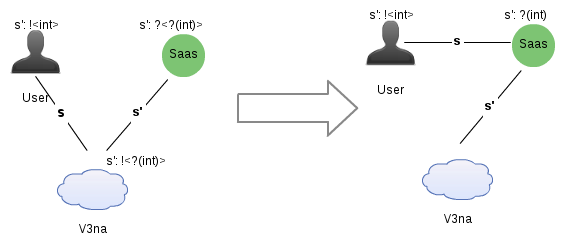
\includegraphics[width=0.8\textwidth]{resources/sj-delegation.png}}
\caption{Session delegation}\label{fig:sj-delegation}
\end{figure}

\paragraph{Protocol Implementation using Session-Java.}
%\paragraph{Another meaning for sockets}
Session sockets represent the participants of a session connection.
Each sockets implement the session code according to the specified session type.
In SJ session sockets extend the abstract \textit{SJSocket} class. %\textit{SJRSocket::SJSocket} and \textit{SJFSocket::SJSocket}.
%Each party owns one endpoint and performs the specified interactions via the SJ session operations on that endpoint.
 %both, employ TCP as underlying transport.
%SJ distinguishes client and server sockets, where the former are used to request sessions from the latter.
%After creating a protocol (session type) and encapsulating the session into SJ socket,
The session is implemented within a session-try scope using specific session operations. %operation  the session operations depicted in Figure \ref{tab:session-ops}.

\begin{comment}
\begin{figure}
\begin{gather*}
\begin{array}{lrl}
s.request() 	&   		    & \mbox{\texttt{begin}} \\
s.send(m)   	&  	 		& \mathopen{!}\left<M\right> \\
s.receive() 	&  	 		& \mathopen{?}\left(M\right) \\
s.outbranch(L) \ \{P\} &  		& \mathopen{!}\left\{L\mathopen{:} T\right\} \\
s.inbranch() \ \{case L1\mathopen{:} {P1}\dots case Ln\mathopen{:}{Pn}\} &   & \mathopen{?}\left\{L_1\colon 
                                        T_1,\dots, L_n\colon T_n\right\} \\
s.outwhile(cond) \ \{P\} 		&   & \left[T\right]\mathopen{*} \\
s.inwhile() \ \{P\} 		 	&   & \mathopen{?}\left[T\right]\mathopen{*} \\
s.recursion(L) \ \{P\} &   & \texttt{rec}\,L\left[T\right] \\
s.recurse(L) &   & \mathopen{\#}L \\
\end{array}
\end{gather*}
\caption{SJ protocol specification}\label{tab:session-ops} 
\end{figure}
\end{comment}

\begin{comment}
\[
\begin{array}{rlrl}
P \Coloneqq & P; P              &                                                               & T_0.T_1 \\
       \mid & s.request() 	&   		    						& \mbox{\texttt{begin}} \\
       \mid & s.send(m)   	&  	 							& \mathopen{!}\left<M\right> \\
       \mid & s.receive() 	&  	 							& \mathopen{?}\left(M\right) \\
       \mid & s.outbranch(L) \ \{P\} &  	                                        	& \mathopen{!}\left\{L\mathopen{:} T\right\} \\
       \mid & s.inbranch() \ \{case L1\mathopen{:} {P1}\dots case Ln\mathopen{:}{Pn}\} &   	& \mathopen{?}\left\{L_1\colon T_1,\dots, L_n\colon T_n\right\} \\
       \mid & s.outwhile(cond) \ \{P\} 		&						& \left[T\right]\mathopen{*} \\
       \mid & s.inwhile() \ \{P\} 		 	&   					& \mathopen{?}\left[T\right]\mathopen{*} \\
       \mid & s.recursion(L) \ \{P\} &   							& \texttt{rec}\,L\left[T\right] \\
       \mid & s.recurse(L) &              							& \mathopen{\#}L \\
\end{array}
\]
\end{comment}

%The session operations are invoked via session in a method call-like manner.
\begin{comment}
\begin{lstlisting}
s1.send(s2) // !<T>, where T is the remaining session type of 's2'
\end{lstlisting}
\end{comment}
To delegate a session, the session socket variable must be passed to a send operation on the target session.
For example, assuming that $s2$ is an active session of type $T$, then the type of $s1.\textit{send}(s2)$ is $\mathopen!\left<T\right>$.
%Only active session sockets can be delegated.
The corresponding receive operation, $\textit{SJSocket}~s2 = s1.\textit{receive}()$ receives delegated sessions.

%------------------------------------------------------------------------------
\section{Case Study: Protocols for a Cloud}
\label{sect:impl}

Our case study is an e-commerce Web portal called V3na that sells SaaS applications for business needs
V3na\footnote{\url{http://v3na.com}. Cloud platform for optimizing your business performance. Source code available at \url{https://github.com/Rustem/Master-thesis}.}
was developed
in the Django framework --- a high-level Web framework for Python. %Further information: \url{https://www.djangoproject.com/}}.
The persistence layer is based on MongoDB and Memcached.
A major challenge was to automate the process of SaaS integration.
In particular, V3na implements the following problems that can be addresses using sessions types:
%By integration, we understand the following processes with a particular SaaS application:
%
\begin{compactitem}
\item  A SaaS user can connect to SaaS for trial period by simply clicking on the button;

\item  V3na provides one entry point to all of the user's applications.

\item  A subscription may be extended or frozen;

\item  The payment for use of a service can be confirmed confirmation;
\end{compactitem}
In this section, we illustrate two refinement of the first scenario above.


\subsection{A Simple Scenario with Branching}
To begin, we specify a simple business protocol for SaaS connection. The protocol is informally specified as follows:
\begin{enumerate}
\item  User begins a request session ($s$) with Cloud service (V3na) and sends the request ``Connect SaaS'' as JSON-encoded message.
\item  V3na sends either:
\begin{enumerate}
\item  FAIL, if user has no active session (not signed in on V3na). % and further interaction terminates 
\item  OK, if user has logged in and request data has passed validation steps. %Then Cloud initiates a new session (s') with SaaS and requests it for new user connection with message details in JSONMsg.
\end{enumerate}
\item  If OK is sent, the Cloud initiates a new session (s') with SaaS and requests it for new user connection with message details in a JSON message.
\item Finally, the SaaS responds to the Cloud with connection status OK or FAIL and V3na sends this status to the user. Both sessions are then terminated.
\end{enumerate}

%Later we will see how decision (choice) in the protocol will be incorporated through the use of dual construct \texttt{outbranch} and \texttt{inbranch}.
%Hence the whole scenario is presented in Figure \ref{fig:protocols-sc1}.
%
{
\lstset{
  framerule=0pt,
  numbers=none,
  basicstyle=\ttfamily\scriptsize,
}
\renewcommand\lstlistingname{Protocol}
\begin{figure}

\begin{minipage}[t]{0.30\textwidth}
\begin{lstlisting}[caption=User]
protocol p_uv { 
  begin.
  !<JSONMsg>. 
  ?{
    OK: ?(JSONMsg).?(int),
    FAIL: 
  }
}
\end{lstlisting}
\end{minipage}
\begin{minipage}[t]{0.35\textwidth}
\begin{lstlisting}[caption=Cloud]
p_vu { 
  begin.?(JSONMsg).!{
    OK: !<JSONMsg>.!<int>,
    FAIL: 
  }
protocol http_req_rep {
  !<JSONMsg>.
  ? (JSONMsg)
}
protocol p_vs { 
  begin.@http_req_rep 
}
\end{lstlisting}
\end{minipage}
\begin{minipage}[t]{0.30\textwidth}
\begin{lstlisting}[caption=SaaS]
protocol p_sv { 
  begin.
  ?(JSONMsg).!<JSONMsg> 
}
\end{lstlisting}
\end{minipage}
\caption{Protocol specifications for Scenario 1}\label{fig:protocols-sc1} 
\end{figure}

In Figure~\ref{fig:protocols-sc1} we depict the protocol specifications for each participant (Cloud, SaaS or User).
The protocols between User and Cloud and Cloud and SaaS are dual, i.e. the specification of interaction from one perspective is opposite from another.

}


%\paragraph{Interactions.} The general syntax for
The global description of the protocol is presented as a sequence diagram in Figure~\ref{fig:interaction-overview-sc1}. %The whole syntax is on the down-left side of the figure.
To represent choice, the OK case is represented by the main picture and the FAIL case is a sub-diagram.
We implement this diagram in Session-Java, where the branching is implemented employing the \texttt{outbranch} and \texttt{inbranch} operations.

\begin{figure}[ht]
\centering
\scalebox{0.3}{
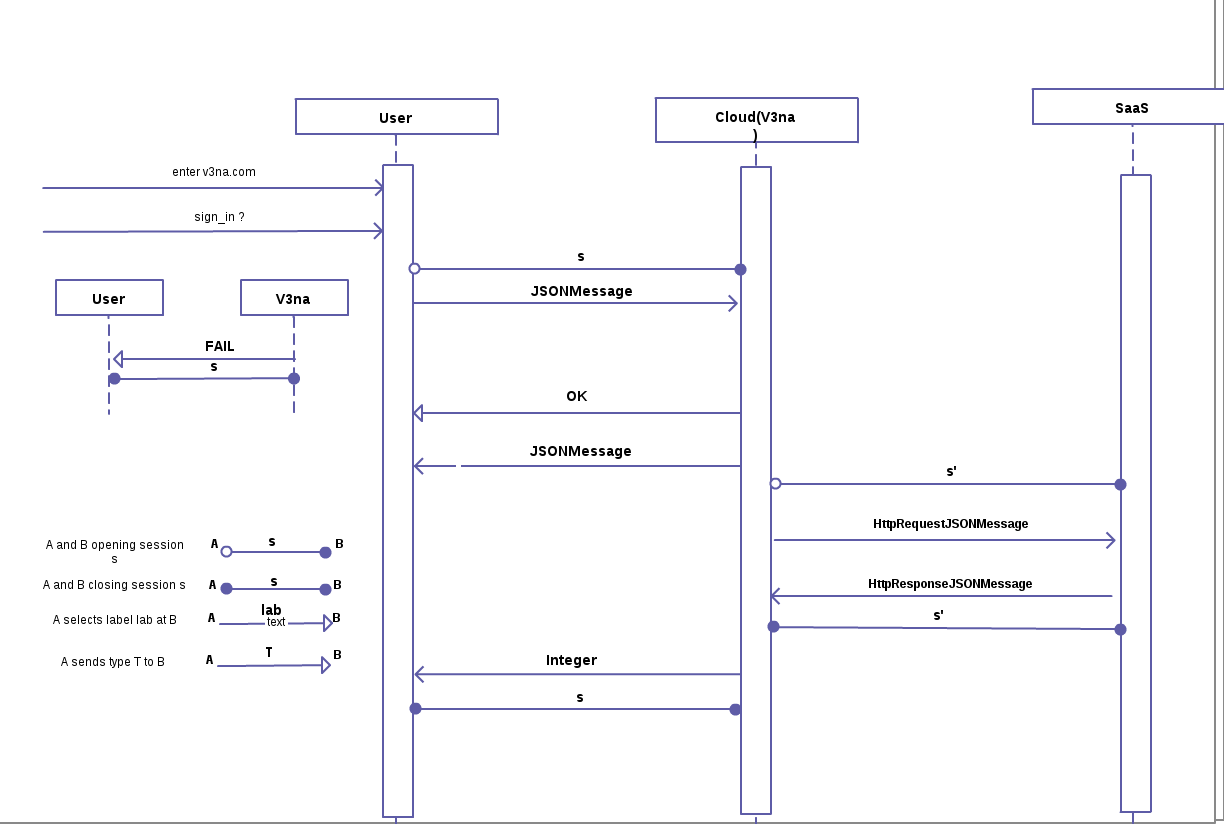
\includegraphics{resources/interaction-sc1.png}}
\caption{Overview of global interactions for Scenario \#1.}
\label{fig:interaction-overview-sc1}
\end{figure}

%\paragraph{Implementation.}


\subsection{The Scenario extended with Iteration}
%New scenario is a bit harder in complexity.
We now introduce the iteration construct and demonstrate \textit{session delegation}.
The informal description of the scenario is as follows:
\begin{compactenum}
\item  User begins a request session ($s$) with cloud service (V3na)

\item  V3na asks User to login, so User provides V3na with login and password.

\item  V3na receives User credentials and verifies them: If User is not authenticated and still has tries%with minimal amount of tries or amount of tries is out of limit,
go back to step 2, otherwise continue.

\item  If User is not allowed to access V3na, the interaction between User and V3na continues on the DENY-branch, otherwise on the ACCESS-branch.

\item  If next branch is ACCESS, User sends his connection request with details to V3na. V3na creates new session with SaaS (s') and delegates the remaining session s with User on the latter and sends last user request details. Session s' is terminated.

\item  SaaS continues interaction with User according to session $s$. By steps of validation-verification, SaaS either responds User to proceed interaction by branch OK or FAIL. In both cases User receives from SaaS directly the reason and status of his request. Eventually, session $s$ is terminated.
\end{compactenum}

%\paragraph{Protocols.}
{
\lstset{
  framerule=0pt,
  numbers=none,
  basicstyle=\ttfamily\scriptsize,
}
\renewcommand\lstlistingname{Protocol}
\setcounter{lstlisting}{0}
\begin{figure}

\begin{minipage}[t]{0.50\textwidth}
\begin{lstlisting}[caption=User]

protocol p_uv { 
  begin.?[!<String>.!<String> ]*.
  ?{
   ACCESS: !<JSONMsg>.
   ?{
     OK: ?(JSONMsg), FAIL: ?(JSONMsg)
   },
  DENY: ?(String)
  } 
}

\end{lstlisting}
\end{minipage}
\begin{minipage}[t]{0.50\textwidth}
\begin{lstlisting}[caption=Cloud]

private protocol p_vu { 
  begin.
   ![ ?(String).?(String) // login password
     ]*.
  !{
    ACCESS: ?(JSONMsg).
    !{
      OK: !<JSONMsg>, FAIL: !<JSONMsg>
     },
      DENY: !<String>
   } 
}

\end{lstlisting}
\end{minipage}
\caption{User-Cloud interaction protocol specifications for Scenario 2}\label{fig:user-cloud-protocol} 
\end{figure}

}

The protocol is specified in Figures~\ref{fig:user-cloud-protocol} and~\ref{fig:cloud-saas-providers}.
The protocol uses iterations specified using $![\dots]*$ and $?[\dots]*$ and higher order operations. % of type $\mathopen{!}\left<T\right>\mathbin{.}\mathopen{?}\left<T\right>$.


{
\lstset{
  framerule=0pt,
  numbers=none,
  basicstyle=\ttfamily\scriptsize,
}
\renewcommand\lstlistingname{Protocol}
\setcounter{lstlisting}{0}
\begin{figure}

\begin{minipage}[t]{0.50\textwidth}
\begin{lstlisting}[caption=Cloud]

protocol p_vs {
  begin.
  !< !{
    OK: !<JSONMsg>, 
    FAIL: !<JSONMsg>
  } >.!<JSONMsg>    
}

\end{lstlisting}
\end{minipage}
\begin{minipage}[t]{0.50\textwidth}
\begin{lstlisting}[caption=Cloud]

protocol p_msg { 
  !{
    OK: !<JSONMsg>,
    FAIL: !<JSONMsg> 
  }
}

protocol p_sv {
  begin.?(@p_msg).?(JSONMsg) 
}

\end{lstlisting}
\end{minipage}
\caption{Cloud-SaaS interaction protocol specifications for Scenario 2}\label{fig:cloud-saas-providers} 
\end{figure}
}

For session type $\mathopen{!}\left<\mathopen{!}\left\{\texttt{OK}\colon \mathopen{!}\left<\textit{JSONMessage}\right>, \texttt{FAIL}\colon \mathopen{!}\left<\textit{JSONMessage}\right>\right\}\right>$, The first ! means that the Cloud is passing the high order message which describes the protocol that Saas should perform with the User.
In the Saas-Cloud protocol, the protocol contains higher order messages by first defining them, then including them in the protocol.
One protocol can be referenced from another using @ operator. %The $@p$ is syntactically substituted for the protocol of that name.

%Unlike the previous protocol, the Cloud-Saas protocol significantly altered, also authentication process is added to the protocol in interaction between User --- Cloud.


\paragraph{Interactions.} Figure~\ref{fig:seq-diagram-sc2} depicts the protocols provided above using a sequence diagram. The language of the artifacts has already presented in the first scenario.

\begin{figure}
\centering
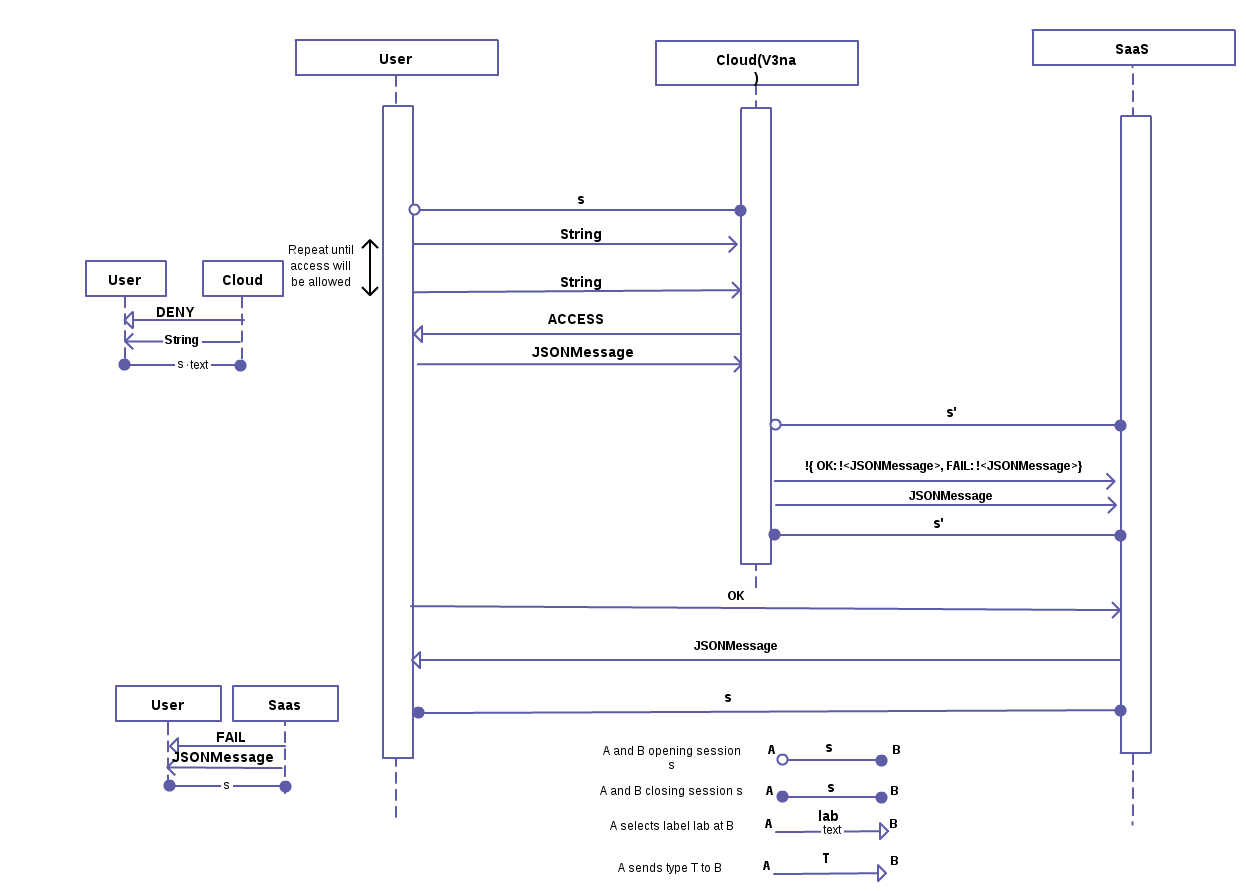
\includegraphics[width=0.8\textwidth]{resources/interaction-sc2.png}
\caption{Sequence diagram of interactions for Scenario \# 2}
\label{fig:seq-diagram-sc2}
\end{figure}

\paragraph{Implementation.} %Despite the fact that session delegation takes place, the program still remains very simple. Actually
Delegating the protocol is straightforward and only consists of passing the socket to service using $\textit{s\_vs}.\textit{send}(\textit{user\_vu})$.
\begin{comment}
\begin{lstlisting}
s_vs.send(user_vu); // pass the remaining protocol
\end{lstlisting}

\begin{lstlisting}
user_vu.outbranch(ACCESS) {
  JSONMessage req_info = user_vu.receive();
  SJServerAddress addr_vs = SJServerAddress.create(p_vs, saas_hname, saas_port);
  SJSocket s_vs = SJRSocket.create(addr_vs); try(s_vs) {
    s_vs.request();
    s_vs.send(user_vu); // pass the remaining protocol    
    s_vs.send(req_info);
  } catch(UnknownHostException uhe) {
    uhe.printStackTrace(); 
  }
}
\end{lstlisting}
\end{comment}

To receive a high order message type casting must take place in the case of a protocol, the type of protocol must be explicitly defined, using $\textit{v3na\_user\_socket} = \left(\mathopen{@}\textit{p\_msg}\right)~\textit{v3na\_sv}.\textit{receive}()$, where \textit{p\_msg} is a defined protocol.
\begin{comment}
\begin{lstlisting}
v3na_user_socket = (@p_msg) v3na_sv.receive();
\end{lstlisting}
\end{comment}
Thus we explicitly define the protocol to be delegated and then include it in the final protocol.

%------------------------------------------------------------------------------


\section{Future Work: InterCloud and Session Types}
\label{sect:highlights}
Cloud computing is moving to the concept where Cloud operated by one enterprise interoperating with a Cloud of another is powerful idea~\cite{Buyya2009}.
So far that is limited to use cases where code running on one cloud explicitly references a service on another cloud. There is no implicit and transparent interoperability. 
Different visions has already proposed in papers~\cite{utility-driven-fed,xmpp-intercloud-transport,cloud-integrator}. The most full picture of cloud inter-networking is depicted by \cite{utility-driven-fed}. They emphasized the main components of general inter-networking architecture:
\begin{inparaenum}[(\bgroup\bfseries a\egroup)]
\item \textit{Cloud Coordinator}, for bringing out Cloud services;
\item \textit{Cloud Brocker}, ``for mediating between service consumers and Cloud coordinators'';
\item \textit{Cloud Exchange} (e.g. Cloud Integrator), for collecting consumers' demands and locating Cloud providers with them with offers.
\end{inparaenum}

Our approach is to employ multiparty session types \cite{ng2012multiparty} for type-safe conversation between Cloud providers and Cloud Integrators (many-to-many conversation). It starts by specifying the intended interactions as an inter Cloud protocol in the, contract checker, UBF. Then processes for each role (either Cloud provider or Cloud Exchange) are implemented in Erlang or Python (they are best for working with high load applications). Since all the roles should be aware of each other in global network in order to dialog with each other, we are going to use SockJS\footnote{SockJS is an effort to define a protocol between in-browser SockJS-client and its server-side counterparts} protocol for presence and AMQP messaging (it's thin, flexible). Moreover, there is an idea, to extend SockJS protocol during communication initiation to check at runtime that each interaction is correct and as a result the whole communication is safe. As a starting point for dynamic verification observers, we referred to \cite{safe-conver-prog-python} work.

\section{Conclusion}
\label{sect:conclusion}
Session-based programming has already proved itself in various fields, including parallel algorithms~\cite{sj-parallel}, event-driven programming~\cite{event-driven-sj} and multi-party conversations~\cite{sj-business-protocols}.
In this paper, our case study demonstrates the ability of session types to control interaction patterns between communicating processes in a Cloud.
Participants are static type-checked at compile time and dynamical type-checking at run-time to ensure that protocol are compatibile.
The higher level of abstraction of session types, implemented in SJ language, enabled effortless translation of business scenarios into protocols.
Support of high-level communication (session delegation), allowed us to refine from Scenario 1 to Scenario 2.
Further to scenarios presented here our case study also covered a scenario involving payment and wallet recharging transactions, %(available by \url{https://github.com/Rustem/Master-thesis}),
where we discovered the benefits of combining session delegation and threading provided in SJ.
The session-programming approach is suited to correctly implementing InterCloud communication protocols, which we intend to test as future work. %Finally, hope that our feedback about session types will be as a solid starting point for further research in this area.  


%------------------------------------------------------------------------------
% Refs:
%
\label{sect:bib}
\bibliographystyle{plain}
%\bibliographystyle{alpha}
%\bibliographystyle{unsrt}
%\bibliographystyle{abbrv}
\bibliography{easychair}

%------------------------------------------------------------------------------
\appendix



%------------------------------------------------------------------------------
% Index
%\printindex

%------------------------------------------------------------------------------
\end{document}

% EOF
